\epigraph{Translation is that which transforms everything so that nothing changes.}{Grass Günter.}

The dream of automatic translation that builds the communication bridge between people from different civilizations dates back to thousands of years (see Fig.~\ref{cp1.fig.babel}). The ability of an algorithm  to translate between any human languages smoothly and accurately has always been a test on whether an artificial intelligence (AI) is capable of understanding human languages. We will start from a brief review of the research of modern automatic machine translation and then move to our main focus: building an {\it efficient} neural machine translation system.

\section{A Brief Review of Machine Translation (MT)}
Researchers have been devoted to proposing practical plans since 1950s.
\begin{figure}[t]
	\centering
	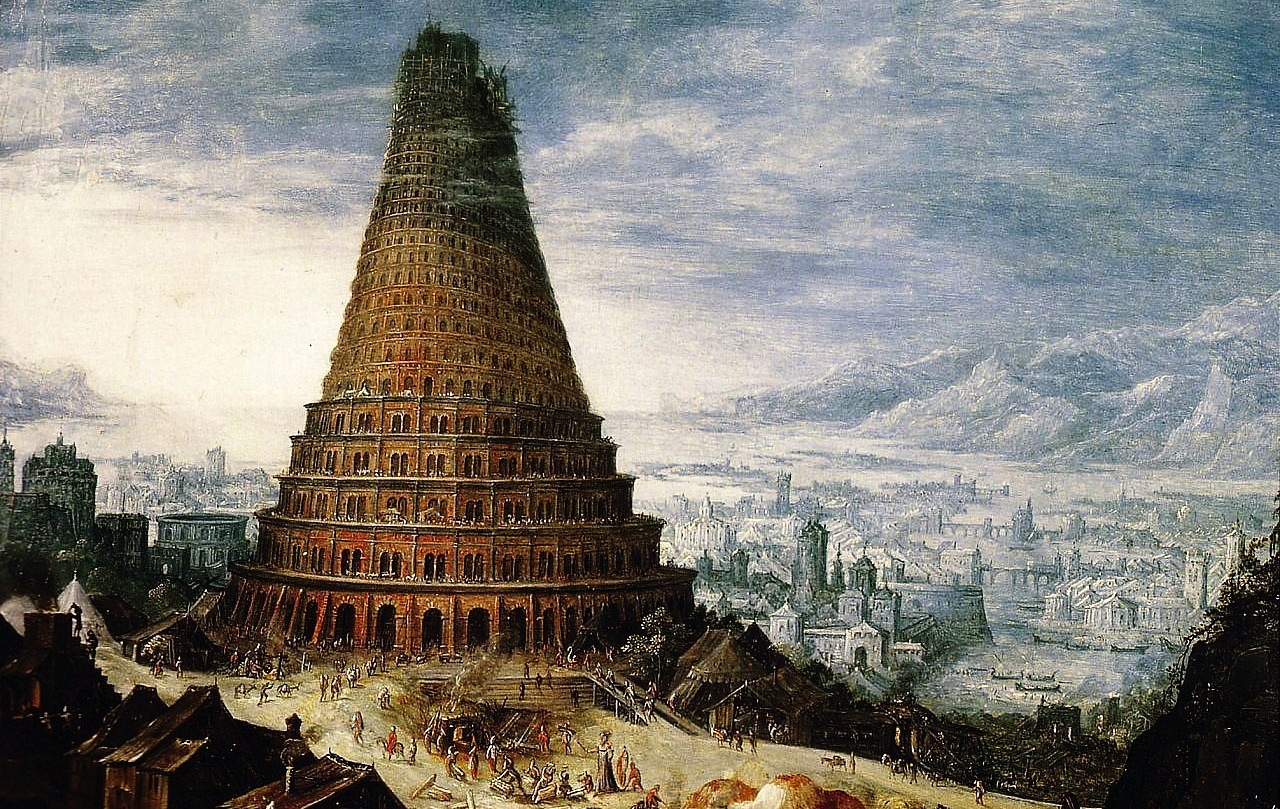
\includegraphics[width=1\linewidth]{figs/intro/tower_of_babel.jpg}
	\caption{\label{cp1.fig.babel}The aim in building Babel and a Tower to “reach into heaven” was to prevent the people from being “scattered abroad over the face of the whole earth” (Genesis 11:4). }
\end{figure}

\paragraph{Rule-based MT} The earliest machine translation systems are rule-based, which requires not only a word-by-word dictionary, but linguists to design specific translation rules language by language. Due to its fragility, the rule-based system easily fails to translate correctly to the countless special cases in human languages, but can usually produce translation with good grammar structure.

\paragraph{Example-based MT}
The example-based machine translation (EBMT)~\citep{Zhang2005AnEP,callison2005scaling,phillips2012modeling} translates new sentences not based on rules, but reference to stored similar translation examples. In a more practical way, it indexes parallel corpora with suffix arrays and retrieves exactly matched translation segments on the fly at test time. %However, to the best of our knowledge, SEG-NMT is the first work incorporating any attention-based neural machine translation architectures and can be trained end-to-end efficiently, showing superior performance and scalability compared to the conventional statistical EBMT. 


\paragraph{Statistical MT} Another trend of machine translation is the statistical machine translation. Similar to EBMT, SMT does not rely on manually mined translation rules. For example, one of the most successful statistical methods,  phrase-based statistical machine translation (PBMT), first builds a phrase table from a large corpora, which later is used to output translation by searching the most proper sequence of paired phrases that fits to an external language model.

\paragraph{Neural MT}
In recent years, with the general success of artificial intelligence (AI) and the emergence of neural network models, a.k.a. deep Learning, neural machine translation (NMT)~\cite{sutskever2014sequence,bahdanau2014neural,vaswani2017attention} , as the new generation of machine translation framework, has achieved the state-of-the-art~\cite{wu2016google} and even human-level translation performance in some languages~\cite{hassan-hp}.
Different from prior work in SMT, NMT does not use an explicit language model, but directly model machine translation as a conditional language model via function approximation.  
The impressive achievements brought by NMT are mainly due to such approximated function, parameterized by deep neural network, 
which can be efficiently tuned from vast volume of parallel data in the order of tens or hundreds of millions of sentences. 

%\begin{figure}[t]
%\centering
%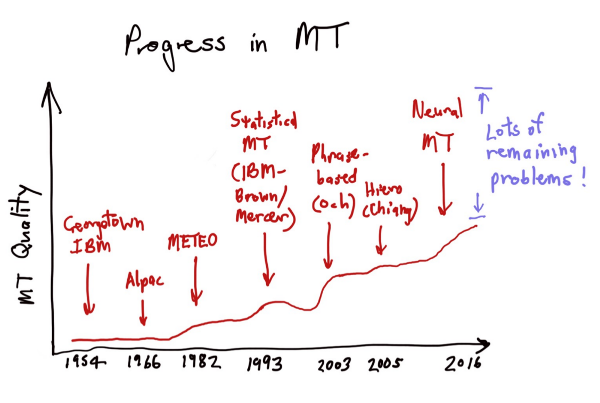
\includegraphics[width=\linewidth]{figs/intro/nmt-history.png}
%\caption{History of machine translation systems. Slide by Christopher D. Manning.}
%\end{figure}


\section{Towards Efficient Neural Machine Translation}

In spite of their success, neural systems also bring about new challenges to machine translation, in which one of the central problems is efficiency. Fundamentally, this ``inefficiency '' of NMT also comes from the deep neural networks which is why  NMT can significantly outperform other solutions. For instance, a standard \footnote{Here we refer to a hyper-parameter settings of  \texttt{t2t-base} reported in the original paper.} of the recently proposed state-of-the-art NMT model  -- the Transformer Model~\cite{vaswani2017attention} -- with a total vocabulary of about $50,000$ subwords requires to learn around $50$ million free parameters from scratch. 
Such huge number of parameters bring about the efficiency issue in two aspects:
\begin{figure}[hptb]
\centering
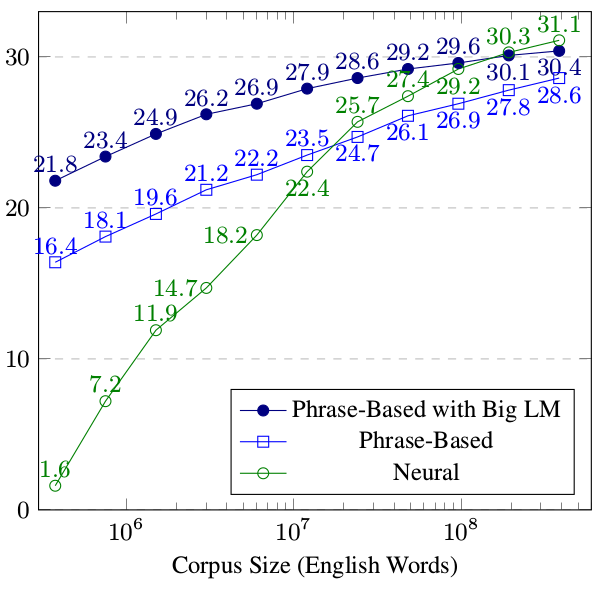
\includegraphics[width=0.6\linewidth]{figs/intro/corpus_size.png}
\caption{\label{cp1.fig.corpus_size} A comparison between NMT and SMT given varying sizes of training examples. Curves extracted from \newcite{koehn2017six}.}
\end{figure}
\begin{itemize}
	\item  It is significantly data-hungry to train these parameters properly using the current (and almost the only) optimization techniques via back-propagation, which makes training a reasonable model difficult in practice for many low resource cases. 
For instance, documents in specialized domains such as law or medical files usually contain tons of professional translations without sufficient examples to remember everything in the network's parameters. Moreover, except for some of the mainstream languages, e.g. English, French or Chinese, most of the human languages lack enough parallel data with other languages to learn a proper NMT model. As shown in Fig.~\ref{cp1.fig.corpus_size}, the poor data-inefficiency of the existing NMT methods compared to traditional methods is also reported as one the most important challenges; 
\item The complicated structure of NMT also makes slow computation (for both training and decoding) compared to other  conventional methods mentioned above. For example, even with the vast speeding-up by the parallelism techniques (e.g. GPUs, TPUs, etc.), because of the restriction of the model assumptions (see details in Chapter~\ref{background} and Chapter~\ref{nat}), decoding sentences by NMT is still 100 or 1000 times slower than SMT or other methods. The low efficiency at inference time profoundly affects the real-life application and the smoothness of the communication. Furthermore, in cases such as video conference or real-time conversion (e.g. see an illustration of simultaneous translation in Fig.~\ref{cp1.fig.simultaneous}), we also hope the neural system to be more efficient so that it can translate at real-time which, however, is difficult for the existing NMT models. 
\end{itemize}
\begin{figure}[hptb]
\centering
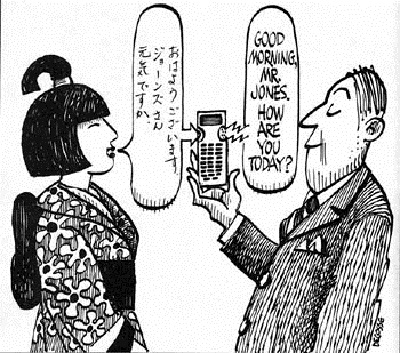
\includegraphics[width=0.6\linewidth]{figs/intro/real_time.jpg}
\caption{\label{cp1.fig.simultaneous}The goal of the efficient NMT decoding -- simultaneous translation.}
\end{figure}
For years, much research has been made for both cases in order to build data and decoding efficient NMT systems. As one of the building blocks of this important trend, this dissertation will specially focus on these two directions, and for each of which we claim 3-4 novel contributions to the field of machine translation research. The detailed outline of this thesis is listed below.

\section{Thesis Outline}
This dissertation attempts to tackle these two challenges discussed above, respectively, with contributions in: {\it data-efficient} (Part \rom{1}) and {\it decoding-efficient} (Part \rom{2}) neural machine translation. 
\begin{itemize}
\item First of all, \textbf{ Chapter~\ref{background}} gives an overview  of  the background for this dissertation,  including the modeling, training and decoding for building a general NMT model. 
\end{itemize}
In Chapters \ref{copy}, \ref{seg-nmt}, \ref{ulr}, \ref{MetaNMT}, we address the data-efficiency challenges presented by existing NMT models and introduce insights based on the characteristics of the data.
\begin{itemize}
\item \textbf{Chapter~\ref{copy}} develops the copying mechanism as a new component  which targets on rote memories in general sequence-to-sequence (\sts) learning. The proposed \copynet also provides a general way in NMT to deal with out-of-vocabulary (OOV) words; 
\item \textbf{Chapter~\ref{seg-nmt}} uses a non-parametric search-engine to search similar translation pairs for guiding the target translation of a standard NMT system. The introduced method can be seen as a direct derivation from \copynet in NMT, but forms a novel non-parametric NMT system that is able to work on translation for professional domains; 
\item \textbf{Chapter~\ref{ulr}} targets on the other direction of data-inefficiency, and invents a universal NMT system for extremely low resource languages. Different from prior works on multi-lingual translation, the proposed methods specially design two additional modules which enable a jointly-trained model to work well on extremely low resource languages with around 6000 sentences; 
\item \textbf{Chapter~\ref{MetaNMT}} extends the previously proposed universal NMT system to enable a pre-trained multilingual NMT model to adapt to any new languages efficiently. Moreover, the usage of meta-learning provides a principled way of finding a better initialization of parameters that is easy to fine-tune on new languages.
\end{itemize}
The second part, Chapters \ref{trainable}, \ref{nat} and \ref{simul}, deal with the decoding-efficiency challenges, and we develop novel structures and learning algorithms.
\begin{itemize}
\item \textbf{Chapter~\ref{trainable}} recasts NMT decoding as a trainable process. The proposed reinforcement learning based algorithm -- {\it trainable greedy decoding} -- not only helps a trained model to decode more efficiently with greedy decoding while achieving better translation quality, but also introduces an interesting direction where we can optimize the decoding towards any favorable objectives.
\item \textbf{Chapter~\ref{nat}} invents the non-autoregressive NMT system that enables translation in parallel. The proposed method, with {\it fertility} as latent variables and sequence-level knowledge distillation, is one of the first NMT systems able to fundamentally remove the restriction of word-by-word decoding in conventional NMT models while keeping a similar translation quality.
\item \textbf{Chapter~\ref{simul}} develops the NMT model that learns to translate in real-time using reinforcement learning. More precisely, we formulate the simultaneous translation as a reinforcement learning setting where two actions -- read and write -- are taken on a pre-trained normal NMT.  The resulted model successfully achieves a balance between delay and quality. 
\end{itemize}
Finally, we conclude and discuss future avenue for efficient NMT in \textbf{Chapter~10}.	 In the next chapter, we will start to introduce in detail the standard NMT models as the necessary background.
